\documentclass[twocolumn]{revtex4}
\usepackage{graphics,graphicx,epsfig,ulem} 
\usepackage{amsmath}
\usepackage{multirow}
\usepackage{gensymb}
\usepackage{commath}
\usepackage{textcomp}
\newcommand{\squeezeup}{\vspace{-2.5mm}}

\begin{document}

\textheight=26.385cm
%Change textheight as the last resort...

\title{Determining the viscosity of water} 
 
 
\author{Jacky Cao, Room 205, Friday, Lab Partners: Peter Dorey, Jon Pritchett \\ Date of experiment: 11/11/2016, Date of report: 20/11/2016}


\begin{abstract}              
 
The volume flow rate of a fluid can be expressed functionally as derived by Poiseuille and Hagen. This relationship can be rearranged so that the viscosity of a fluid can be experimentally determined. By performing analysis of data of the mass, volume, and heights, it is possible to calculate the viscosity of water, $\eta_{water}$. The average value obtained was determined to be $1.00 \pm 0.03$ mPa s which does not agree with the literature value, $1.679$ mPa s. [[mention accepting and why??]]

\end{abstract}

\maketitle

\section{Introduction} 
\vspace{-2ex} 

Derived experimentally by Poiseuille in 1838 and Hagen in 1839 \cite{poiseuillehagen}, the volume flow rate $dV/dt$ of a fluid passing through a tube can be expressed as a function of the density of the fluid $\rho$, the value for acceleration due to gravity $g$, the height the fluid leaves the tube $h$, the radius $a$ and length $L$ of the tube, and the viscosity of the fluid $\eta$,

\squeezeup

\begin{equation} 
\frac{dV}{dt}=\frac{\pi}{8}\frac{\rho gh}{\eta}\frac{a^4}{L}. 
\label{pohagen}
\end{equation}

Noting that the group $\rho gh$ can be collectively termed the pressure difference $\Delta P$ between the two ends of the tube \cite{collegephysics}. [[?? add something more to here]]

If we consider that a fluid is flowing through said [[?]] tube, it experiences both friction with the inner wall and internal friction within itself. The latter can be defined more readily as the viscosity of the fluid $\eta$, and this results in shear stress when two adjacent layers (laminas) of fluid move relative to each other. 

We find that as $\eta$ increases, the volume flow rate decreases, the shear stress between two laminas becomes greater and so restricts the movement of the fluid's molecules trying to flow through the tube. 

Generally we can say that the lamina flow streamlines are smooth, top layers sliding over other laminas without the system having any turbulent motion - this condition is required for equation (\ref{pohagen}) to be valid. 

Using a rearranged form of the relation derived by Hagen and Poiseuille, and making various initial assumptions it is possible to experimentally calculate a value for the viscosity of water. Our assumptions being that the fluid is incompressible, the temperature of the water does not change, and the flow rate of water is something [[?]].

\vspace{-3ex}
\section{Method} 
\vspace{-2ex}
A flow of water was created by fixing a capillary tube to a water tank. The tank was raised to an initial height arbitrary height above the work surface[?]. The tank was then filled up with water from heights ($h$) 2cm to 16cm at 2cm intervals, these values were measured with the markings on the side of the tank. During this we had to ensure that we did not create parallax between the level of the water and the markings on the side. 

The water was then allowed to flow out of the tube for a period of 90s for each height of water, this time was measured using a digital stopwatch. As the water flowed out it was caught within a large beaker so that the mass and volume of it could be measured after the allotted time had passed. 

The mass was found by having the beaker already on a set of electronic scales and initially zeroed to account for the beaker's mass. The volume on the other hand required the water to be transferred from the beaker to a measuring cylinder, this was performed by using a pipette. Care was again taken so that there was no parallax and that no unaccounted water was left within the beaker. It was also necessary to clear the tube once air bubbles formed along the length of it this was done using a long piece of copper wire. 

\begin{figure}[!h]
\begin{center}
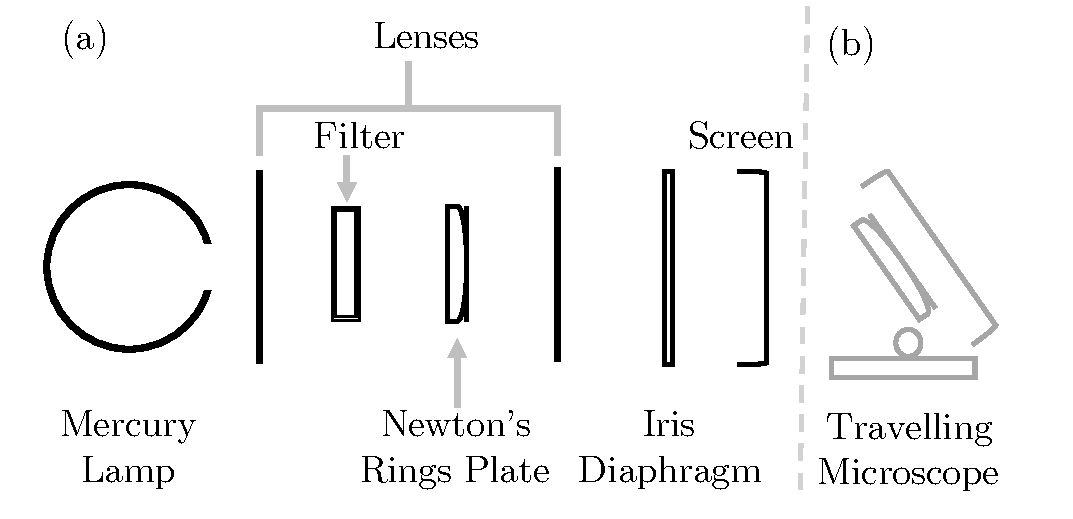
\includegraphics[width=5.7cm]{fig1}
\caption[]{A schematic of the experimental set-up used to collect data. }
\label{fig:fig1}
\end{center}
\end{figure}

\squeezeup
\squeezeup

An initial density value for water was calculated by taking four measurements of the volume and mass of the water, then calculating four values for $\rho_{water}$, and then averaging it so find a value. 

One set of data was taken for each of the three capillary tubes that were used. Each tube varied in their internal diameter, $d$, this was measured using a travelling microscope along the horizontal axis. 

The collected data was applied to a least squares fitting to create an initial linear model, $dV/dt$ as a function of $h$. This was then used to calculate the flow rate for each different height, and also allowing us to perform analysis of the data.

\vspace{-3ex}
\section{Results}
\vspace{-2ex}

The volumetric flow rate of water is plotted against the varying height, as shown in Fig. \ref{fig:fig2}. This flow rate was calculated by dividing each value of the measured volume with the measured time period. Using this data, a value of viscosity could be calculated through a rearranged form of equation (\ref{pohagen}),

\squeezeup

\begin{equation} 
\eta=\frac{\pi \rho g a^4 }{8 L m}, 
\label{r-pohagen}
\end{equation}

where $m$ is the gradient of the least squares regression line, calculated with the known data for $dV/dt$ and $h$.

From preliminary results taking, our density of water is ${1001 \pm 1}$ kgm$^{-3}$, this was used in later calculations.

The calculated values for the viscosity of water are shown in Table \ref{table:1} with which respective tube was used, the radius (found by dividing $d$ by two), the reduced $\chi^2$ statistic, and the Durbin-Watson statistic ($\mathcal{D}$) for each of those tubes. 

An average value for viscosity can thus be found to be $1.00 \pm 0.03$ mPa s, which does not agree with the literature value \cite{crc}, $1.679$  mPa {s}. 

\vspace{-1ex}
\begin{figure}[!h]
\begin{center}
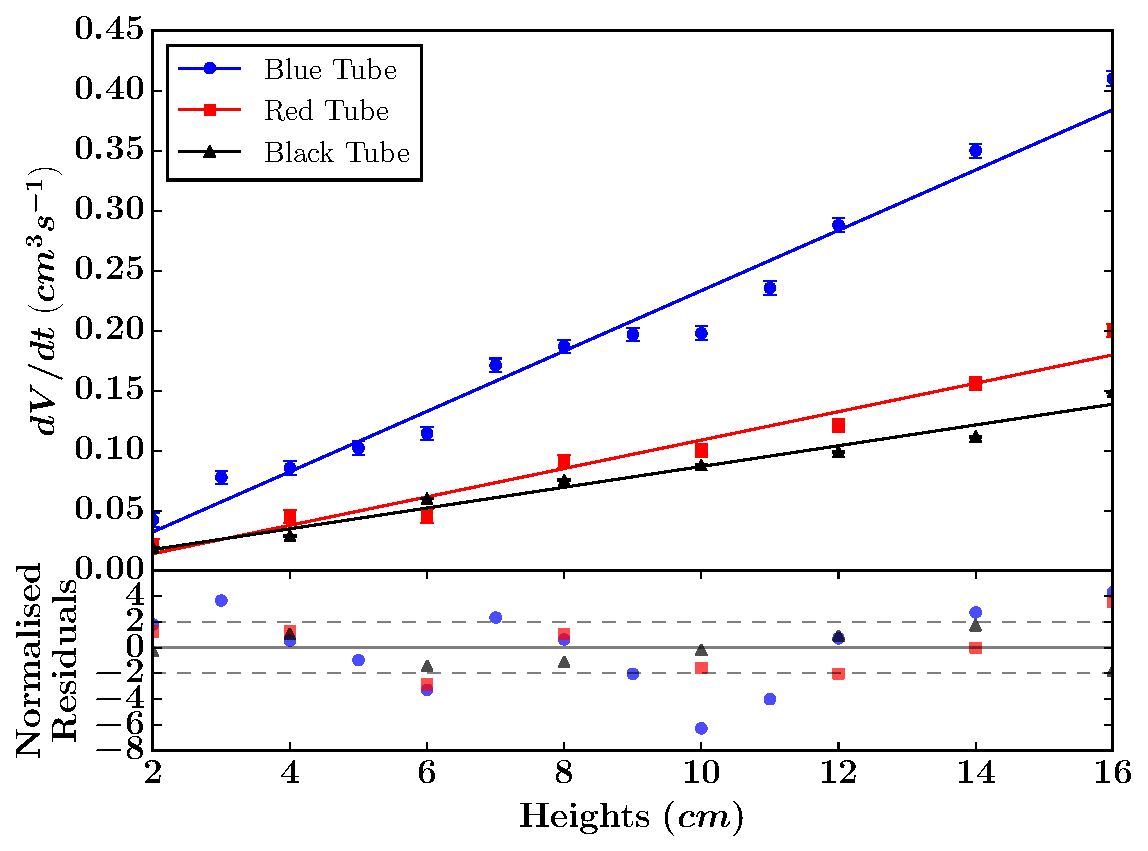
\includegraphics[width=9cm]{fig1-3}
\caption[]{The volume flow rate of water ($dV/dt$) as a function of height ($h$) for three capillary tubes of different diameter. The vertical error bars on $dV/dt$ are too small to be seen.}
\label{fig:fig2}
\end{center}
\end{figure}

\squeezeup
\squeezeup
\squeezeup

\begin{table}[h!]
\centering
\begin{tabular}{ |c|c|c|c|c| } 
 \hline
 \textbf{Tube} & \textbf{Radius, a [mm]} & \textbf{$\boldsymbol{\eta_{water}}$ [mPa {s}]} & \textbf{$\boldsymbol{\chi^2_{\nu}}$} & $\mathcal{D}$\\ [0.5ex] 
 \hline\hline
 $Blue$ &$0.55\pm0.03$ & $1.0\pm0.2$ & 11.0 & 1.11\\ 
 $Red$ & $0.47\pm0.03$ & $1.1\pm0.3$ & 5.31 & 2.20\\
 $Black$ & $0.46\pm0.03$ & $1.0\pm0.3$ & 1.94 & 2.91\\
 
 \hline
\end{tabular}
\caption{Radius of the three tubes, their respective calculated value for $\eta_{water}$, the reduced chi-squared statistic, $\chi^2$, and the calculated Durbin-Watson statistic, $\mathcal{D}$, is shown for each tube as well.}
\label{table:1}
\end{table}

\squeezeup
\squeezeup

\vspace{-3ex}
\section{Discussion}
\vspace{-2ex}
From an initial inspection of Fig. \ref{fig:fig2} we see that the change in $dV/dt$ with $h$ appears to follow a linear regression model. However, we can see that the majority of the error bars for all three sets of data do not seem to be within the range of the lines of best fit. This could mean that our data is not entirely accurate and further experimentation may be required. 

We can further explore the validity of our data by looking at the calculated reduced chi-squared and Durbin-Watson statistics. A reasonable fit to the model should expect $\chi^2_{\nu}$ and $\mathcal{D}$ to be approximately one and two respectively \cite{hughesandhayes}. For our data, we see that the black tube has the closest $\chi^2_{nu}$ value to unity, so from this statistic this set of data has the best fit to the model. However, this tube also has the greatest difference from two, implying that while the fit is not bad, it is not the best. 

From our data we can see that all three values of $\eta$ do agree with each other within their experimental errors. Although, the calculated value for the viscosity using the blue tube has the biggest disparity when compared with the literature value. While the 'Solver' function was used on Excel to try and reduce the $\chi^2_{\nu}$ value, it is still remains fairly large. This could be because the radius of this tube is the greatest out of all three tubes, so the volume flow rate would also be the greatest, thus the amount of water being collected would increase, resulting in difficulties in accurately measuring the mass and volume of it.

With our experimentation, we can consider that there were some limitations with how our data was collected. For the volume of the water, it was likely that the $V$ we measured was not the actual value that had flowed out of the tank. This problem arose due to the fact that some water was left within the pipette when transferring from beaker to the measuring cylinder, and the capillary tube would not form a perfectly air tight seal with the tank so water leaked out.

Another experimental limitation was that the diameter of each tube was not uniform throughout. With this, we find that due to the tapering of the tube the volume flow rate would have been reduced as the flow of the water would have been non-uniform.

Other factors were not taken into account during our calculations such as the variation in the density of water with temperature change. From the Thiesen-Scheel-Diesselhorst equation \cite{dentemp}, we see as the temperature of water increases, the density of it decreases, meaning that the viscosity will decrease as a result. While we assumed that the fluid was incompressible, our calculations could be altered to account for this and thus potentially produce a more accurate result for $\eta_{water}$.

For our experiment we also took only one data set for each tube as we were limited by time. One certain improvement for our experiment would be to take repeat measurements for each tube so that the standard error can be calculated for each tube.  

\vspace{-5ex}
\section{Conclusions}
\vspace{-2ex}
 
In conclusion, through experimentation it is possible to calculate values for the viscosity of water which are similar to [[The experiment was limited by difficulties in measurement, the amount of data unable to be taken - more data could have been taken to account for the temperature change maybe. Also repeat measurements so the mean and standard error could be used instead of trying to calculate values yourself. More time needed so more data, in the time given, only one set of data was taken for each tube so that different flow rates could be considered. ]]

\squeezeup
\squeezeup

\begin{thebibliography}{5}
\bibitem{poiseuillehagen}
	Salvatore P. Sutera and Richard Skalak
	\textit{The History of Poiseuille's Law}.
	Annu. Rev. Fluid Mech., 1993.
	
\bibitem{collegephysics}
	Raymond A. Serway, Chris Vuille, and Jerry S. Faughin
	\textit{College Physics, 8th Edition}.
	Brooks/Cole, Belmont, CA, USA, 2009.

\bibitem{youngandfreedman} 
	Hugh D. Young and Roger A. Freedman.
	\textit{University Physics with Modern Physics, 13th Edition}. 
	Pearson Education Limited, Essex, UK, 2015.
	
\bibitem{crc} 
	David R. Lie
	\textit{CRC Handbook of Chemistry and Physics, 84th Edition}. 
	CRC Press, Florida, USA, 2004.
	
\bibitem{dentemp} 
	J. L. Martin and S. C. McCutcheon
	\textit{Hydrodynamics and Transport for Water Quality Modelling}. 
	CRC Press, Florida, USA, 1999.
	
\bibitem{hughesandhayes} 
	I. G. Hughes and T. P. A. Hase
	\textit{Measurements and their Uncertainties}. 
	Oxford University Press, Oxford, UK, 2010.
	
\end{thebibliography}
\clearpage

\vfill
\twocolumngrid
\vspace{-3ex}
\section*{Appendix}
\vspace{-2ex}

WIP

\clearpage
\end{document}